\chapter{Problem Statement and Solver Methods}
\label{sec:solver}

In the following, the problem to optimize will be introduced an analyzed.
Although the thesis is not looking into finding the optimal solution, different solver strategies have to be introduced and compared to each other, as the utility function is not trivial and the differences are severe.
Their advantages and disadvantages will be shown.
If not specific mentioned, we will look at a 2x2 MIMO system with one receive antenna per user and three relays, as shown in Figure~\ref{fig:antenna_placing}.
The relays in this system will be lossless, i.e. the impedances will be pure imaginary.

\section{Utility Function}
\label{sec:utility_function}
As the aim for wireless communication networks is to maximize the achievable rate, we take the formulas derived in Section~\ref{sec:rates}, which describe the rates for each transmit-receive pair.
In order to get an utility function from the achievable rates, we take the vector of achievable rates $\vec{r} = \begin{bmatrix}
r_1 & r_2 & \cdots & r_N
\end{bmatrix}^T$ from Equation~\eqref{eq:achiev_vec}.

To optimize the rates, different approaches are possible.
\begin{itemize}
\item Optimize the minimum rate, i.e. $\text{max}\left(\text{min}(\vec{r})\right)$ (maxmin), and
\item Optimize the mean rate, i.e. $\text{max}\left(\sum(\vec{r})\right)$ (maxsum)
\end{itemize}

This is done using the LP-norm ($||\vec{r}||_p$)~\cite[p.853]{Kreyszig}.
By setting $p = -\text{Inf}$, the "maxmin" method is achieved.
Setting $p = 1$, the "maxsum" method is applied
For all values in between, the utility function "tends" to optimize the sum and the minimum value respectively.
In the following we restrict ourselves to the "maxsum" method.
As the other methods easily can be applied and will lead to a similarly good result without loss of generality.

\subsection{Convexity of the Utility Function}
\label{sec:}

In the following the convexity of the utility function is analyzed.
This is done, because the choice of the solver depends on the shape of the utility function (e.g. in case of a concave utility function, a normal gradient search is sufficient to provide good results).
\begin{figure}[h]
\centering
  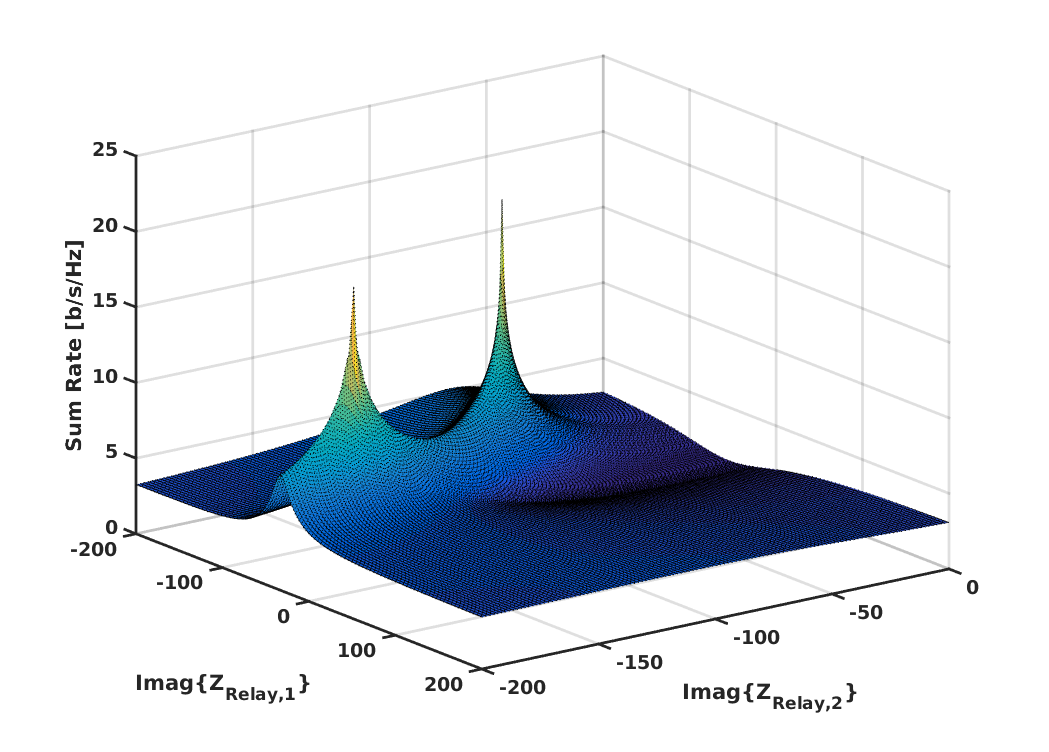
\includegraphics[width=0.8\linewidth]{images/full_mesh_highsnr_93.png}
\caption{The utility function for a specific channel realization.}
\label{fig:utility_power1}
\end{figure}

To do so, we analyze the utility function at different input values for the passive relays.
It is clear, that the function (heavily) changes for every channel realization.
Figure~\ref{fig:utility_power1} and~\ref{fig:utility_power2} show two different channel realizations for the same input power and the same domain of two passive impedances.


For the domain of the relay values showed in Figure~\ref{fig:utility_power1}, even two local maxima could be found, with an immensely higher sum rate value.
On the other hand, the utility function in Figure~\ref{fig:utility_power2} shows only one local maximum with such a huge performance difference. 


\subsection{Dependency on the Input Power}
\label{sec:}

We will analyze now the utility function for different input powers.
In Figure~\ref{fig:utility_power2} and Figure~\ref{fig:utility_power3} we see the same channel realization for two different input powers.

\begin{figure}[h]
\centering
  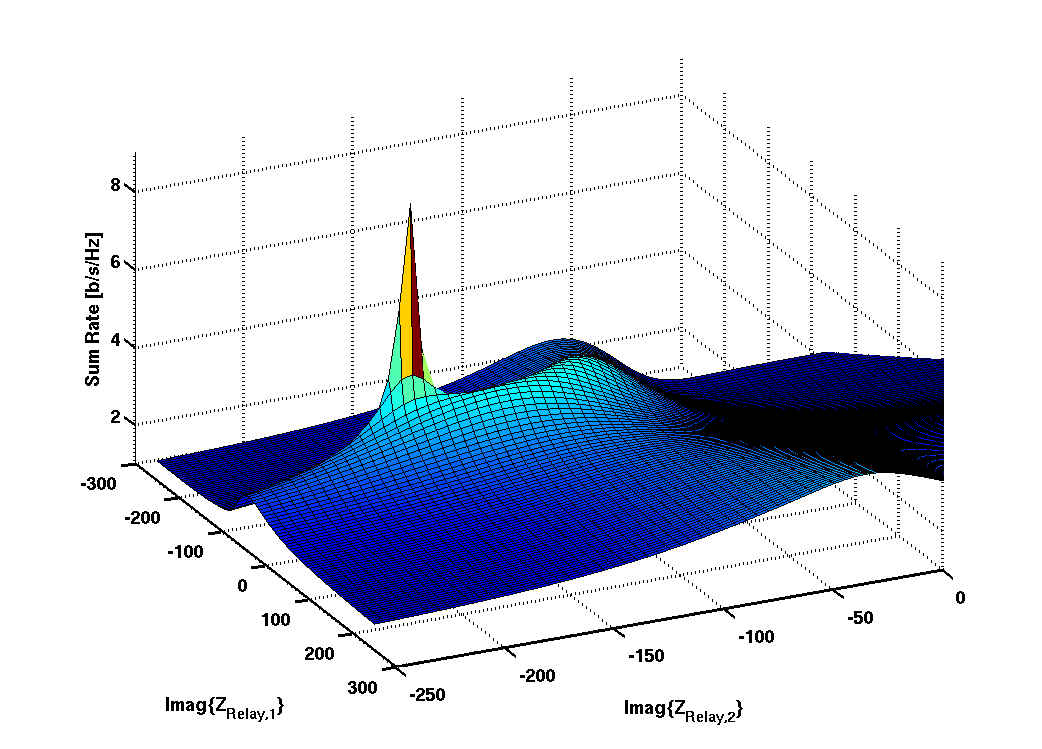
\includegraphics[width=0.8\linewidth]{images/full_mesh_highsnr_99.png}
\caption{The utility function for an other specific channel realization and a high input power level.}
\label{fig:utility_power2}
\end{figure}

We observe, that the optima in Figure~\ref{fig:utility_power2} and Figure~\ref{fig:utility_power3} lie at different impedance values of the relays, therefore we can conclude, that an optimal solution for one input power does not necessarily lead to a good solution for a different input power solution.

\begin{figure}[h]
\centering
  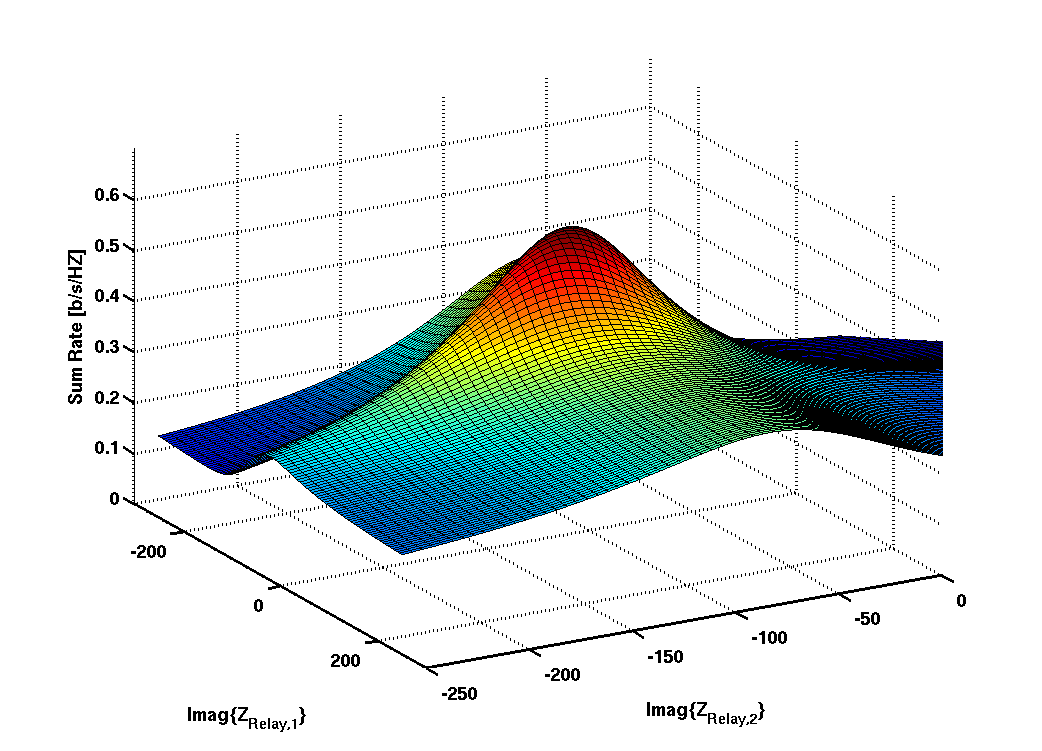
\includegraphics[width=0.8\linewidth]{images/full_mesh_modsnr_99.png}
\caption{The utility function for the same specific channel realization as in Figure~\ref{fig:utility_power2} and a moderate input power level.}
\label{fig:utility_power3}
\end{figure}

\subsection{Difference of Local Optima}
\label{sec:}


Last, we want to look at the local optima we can possibly run into.
We see in Figure~\ref{fig:utility_power1}, that if we hit the local optimum at the left, the performance will be nearly the same as with the local optimum at the right.
However looking at Figure~\ref{fig:utility_power4}, we see that the difference of the global optimum of the section shown is with above 18 [b/s/Hz] severly higher than the local optimum on its left with around 8.5 [b/s/Hz].
Therefore, we can not only try to run the optimization with one initialization, but instead, we need multiple initializations, to be sure, that we haven't missed a sever maximum.
\begin{figure}[h]
\centering
  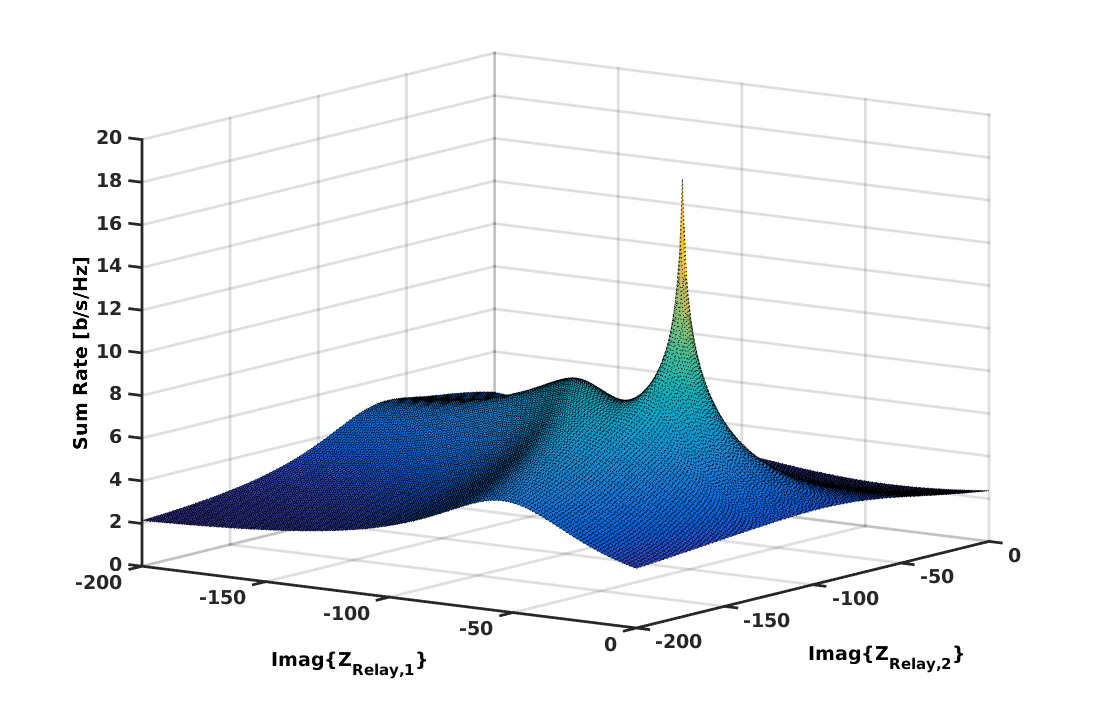
\includegraphics[width=0.8\linewidth]{images/full_mesh_highsnr_94.png}
\caption{The utility function for a specific channel realization.}
\label{fig:utility_power4}
\end{figure}

\subsection{Complexity of the Problem}
\label{sec:}

As we will discuss different solver approaches in the following Sections, a short description of the complexity of the problem is given.
For each relay we use, we will have one variable ($N_\text{Rel}$), if we restrict the relays to the imaginary domain.
Allowing the relay to become lossy and therefore the impedance complex, the number of variables is doubled.% ($2\cdot N_\text{Rel}$).
Further for each receiver branch, i.e. receiver antenna, we have a reciprocal (lossless) matching network (see Section~\ref{sec:matching_network}), which has to be optimized.
Therefore we have three elements per branch (in total: $3\cdot N_\text{R}\cdot N_\text{Rx}$).
For a four user MIMO system with two receive antennas and five lossy relays per user, this would lead to a problem of size $N_\text{var} =  2\cdot 4\cdot 5 + 3\cdot 4\cdot 2 = 64$.
As mentioned in the beginning of this chapter, we look at a 2x2 MIMO system with one receive antenna and three lossless relays.
The complexity of this system is therefore $N_\text{var} =  1\cdot 2\cdot 3 + 3\cdot 2\cdot 1 = 12$.

\section{Gradient Search}
\label{sec:grads_solver}

Despite this large number of variables and the non-convexity of the utility function, the first approach remains a gradient search.
Figure~\ref{fig:grad_search} shows the typical behavior of the gradient search versus the iteration steps.
In the following, different methods are described, to improve the algorithm.

\begin{figure}[h]
\centering
  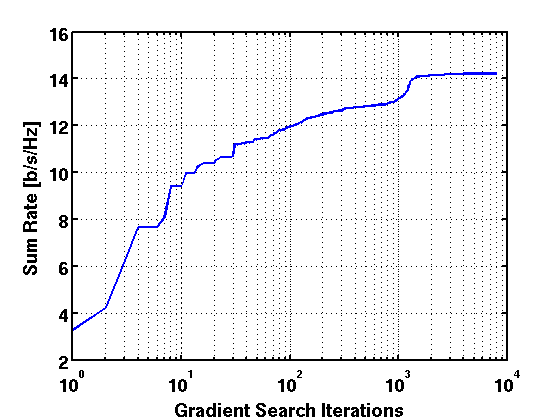
\includegraphics[width=0.8\linewidth]{images/rvsgradCnt_7rel_18dB_6.png}
\caption{The sum rate over the gradient search iterations.}
\label{fig:grad_search}
\end{figure}

From Figure~\ref{fig:grad_search}, it is also obvious to see, why the method of gradient search was taken despite the non-convexity of the problem:
The rate is tripled after seven steps, and after 100 steps the rate is improved by a factor of four.
Afterwards only small improvements can be achieved, which leads to the assumption, that a sufficiently good local maximum can be found very fast.
If after such a small number of steps no good result can be achieved, it leads to the assumption, that the initial value was poorly chosen, hence with a different initialization a better result might be achieved.
This is also shown in the following section.

\subsection{Choice of Initial Values}
\label{sec:grads_ini}
We try to overcome the non-pleasant properties of the problem with a larger number of initial guesses, so that the gradient search approach tends more towards a grid search optimization method.
The gradient search routine itself is then used as a refinement step of the grid search.
%(c.f. \cite{Adjashvili2012})
\begin{figure}[h]
\centering
  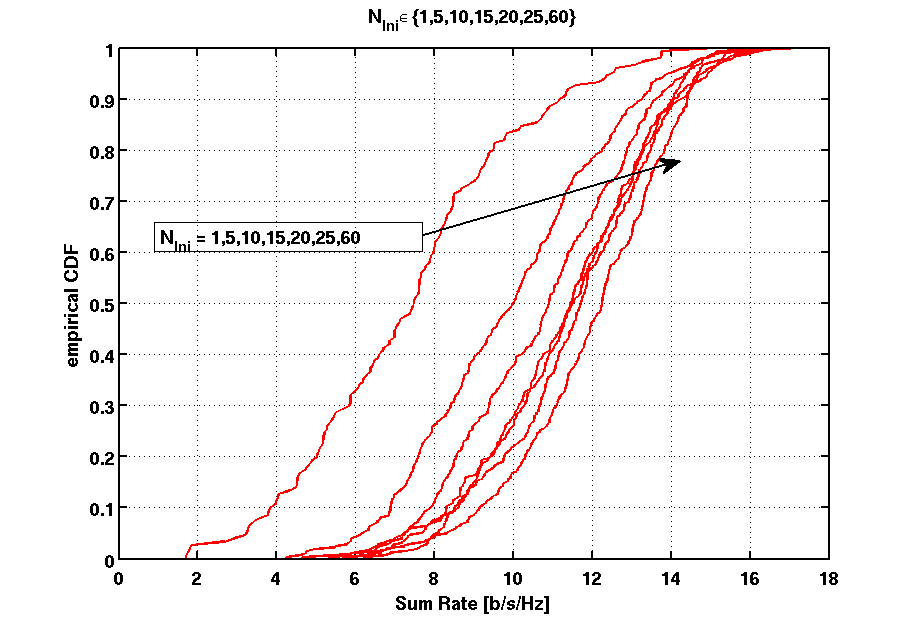
\includegraphics[width=0.9\linewidth]{images/Inicomparison_edited.png}
\caption{Comparison of the number of initial values used.}
\label{fig:ini_comp}
\end{figure}


Figure~\ref{fig:ini_comp} shows the empirical CDFs of the optimized sum rate, for different numbers of initializations.
The initial values were drawn uniformly at random for $Z_{\text{Rel}}[i]\in[-600,600] j , \quad\forall i\in[1,N_{\text{Rel}}]$.

It is obvious and clear to see, that the larger the number of initializations, the better the result.
However, even with 25 and 60 initializations, there improvement is still immense, which shows, that the number of initializations must be a lot larger than twice the input vector length.
A good tradeoff between a decent optimization and a comparable small run time of the optimization is achieved by a choice of four times the input vector length.
\begin{figure}[h]
\centering
  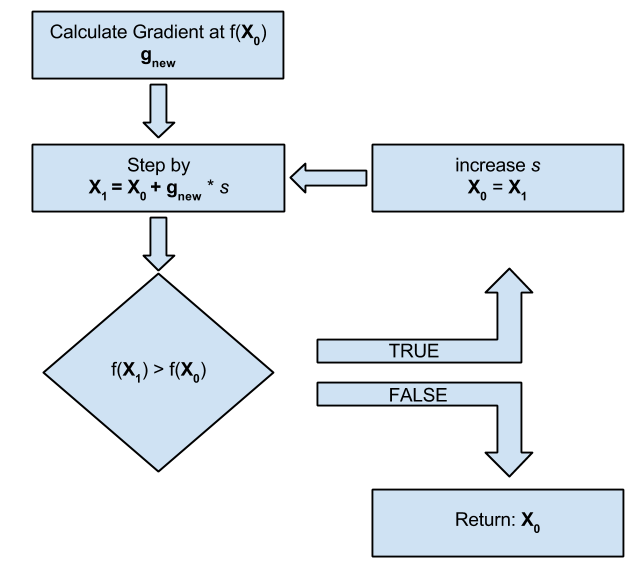
\includegraphics[width=0.5\linewidth]{images/stepsize_scheme.png}
\caption{Schematic of the adaptive step size algorithm.}
\label{fig:stepsize}
\end{figure}

\subsection{Adaptive Step Size}
\label{sec:grads_stepsize}
The performance of the gradient search routine is improved by the use of an adaptive step size.
For each calculated gradient, the step taken into the direction of the gradient is increased until the new rate value is smaller than the previous calculated value as shown in Figure~\ref{fig:stepsize}.
Therefore the number of time-expensive gradient calculations is reduced immense.



\subsection{Conjugate Gradient}
\label{sec:grads_conjgrad}
\begin{figure}[h]
\centering
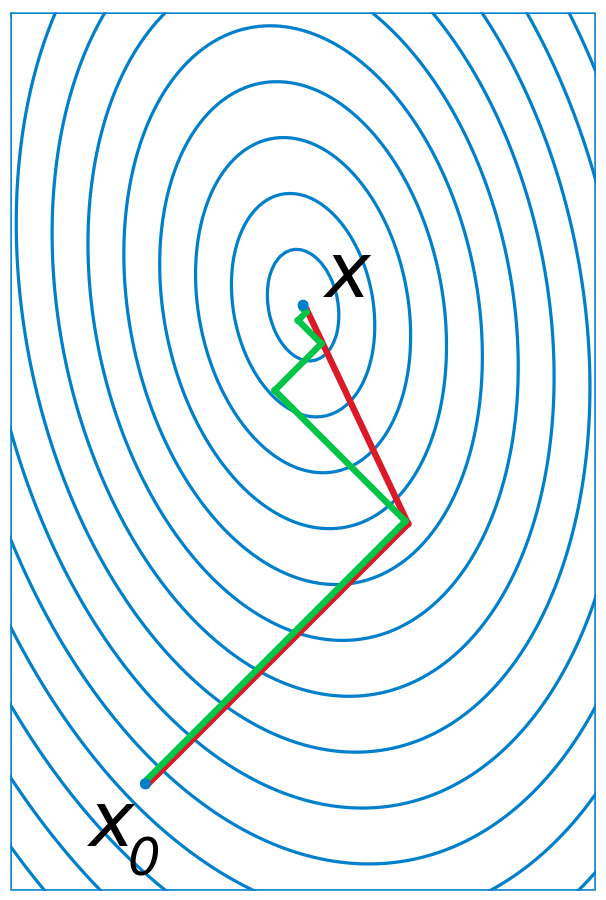
\includegraphics[width=0.25\linewidth]{images/conjugate_gradient_example.png}
\caption{A comparison of the convergence of gradient descent with optimal step size (in green) and conjugate vector (in red) for minimizing a quadratic function associated with a given linear system\cite{wiki:conj_grad}.}
\label{fig:conj_grad_ex}
\end{figure}
As the gradient search performance still requires too many iterations, further improvements were made.
The shape of such complex problems can - in some cases - have the shape of a crest, where, with a unpleasant choice of the initial value, a pure gradient search routine might jump around the optimum, without improving a lot.
Conjugate gradient routines like "Fletcher-Reeves" or "Polak-Ribi\`{e}re" lead to a faster convergence, as they weight the gradient by the previous gradient and a weigth factor $\beta$. 

Like Polak-Ribi\`{e}re, the Fletcher-Reeves method updates the conjugate direction according to 
\begin{equation}
\vec{s}_n = \vec{g}_n + \beta_n\cdot\vec{s}_{n-1},
\label{eq:conj_update}
\end{equation}
where $\vec{g}$ denotes the gradient.
The conjugate direction $\vec{s}$ is then used to perform the conjugate gradient search.
Polak-Ribi\`{e}re and Fletcher-Reeves differ in the way, they calculate the weight factor $\beta$.

\subsubsection{Fletcher-Reeves}
For the method of Fletcher-Reeves, $\beta$ is calculated according to~\cite{Fletcher64}
\begin{equation}
\beta_n^{FR} = \frac{\vec{g}_n^T \vec{g}_n}{\vec{g}_{n-1}^T \vec{g}_{n-1}}.
\label{eq:beta_fr}
\end{equation}

\subsubsection{Polak-Ribi\`{e}re}
For the method of Polak-Ribi\`{e}re, $\beta$ is calculated according to~\cite{Polak69}
\begin{equation}
\beta_n^{PR} = \frac{\vec{g}_n^T\left(\vec{g}_n-\vec{g}_{n-1}\right)}{\vec{g}_{n-1}^T \vec{g}_{n-1}}.
\label{eq:beta_fr}
\end{equation}

\begin{figure}[h]
\centering
  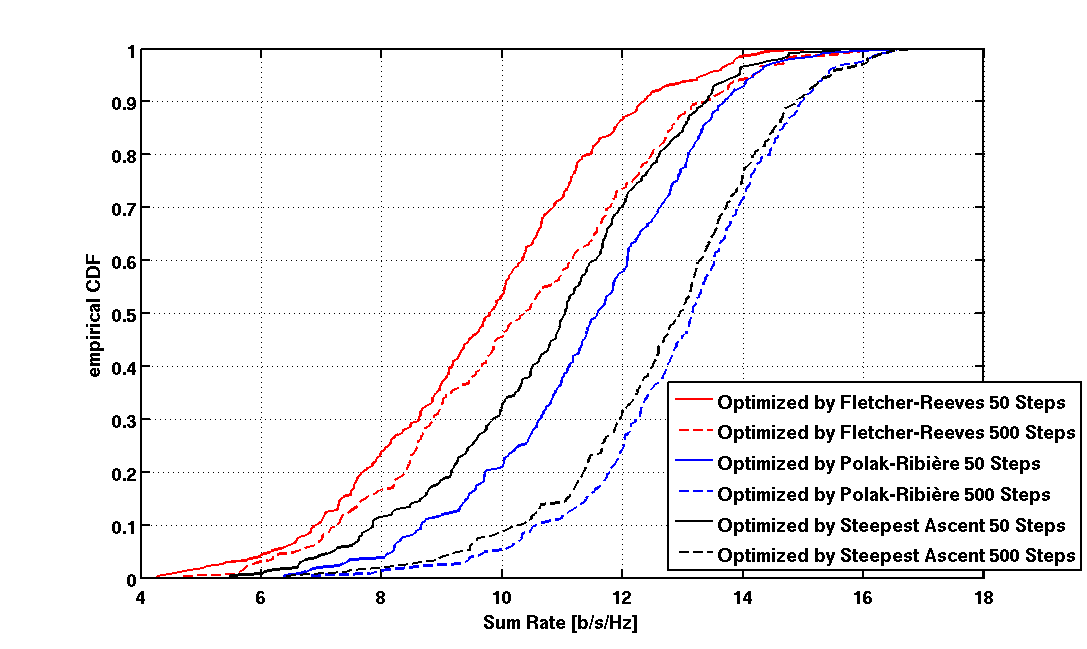
\includegraphics[width=0.8\linewidth]{images/Conjgradcomparison_edited.png}
\caption{Comparison between Steepest Ascent, Polak-Ribi\`{e}re, and Fletcher-Reeves.}
\label{fig:pr_fr_sa}
\end{figure}

In Figure~\ref{fig:pr_fr_sa} the pure gradient search (steepest ascent) method is compared to the methods of Fletcher Reeves and Polak-Ribi\`{e}re.
The Figure shows once the optimization after 50 iterations (solid lines), to see, which method optimizes the problem the best after just a few steps, and at 500 iterations, to see which routine might get caught in the shape  of the problem.


We can see, that Fletcher-Reeves is not well suited for our kind of optimization problem.
Better is Polak-Ribi\`{e}re, which outperforms the standard gradient search method at 50 iterations and has a slightly better performance at 500 iterations.


\section{Heuristic Optimization Algorithms}
\label{sec:heuristic}
Due to the non convexity and the non trivial optimization problem, we further analyze (some) heuristic optimization methods.
In the following three heuristic algorithms will be introduced and analyzed by their performance.
They were chosen, because they already exist in the MATLAB library and do not require any strenuous implementation.

\subsection{Simulated Annealing}
\label{sec:sim_annealing}
Simulated Annealing was developed, as there is a deep and useful connection between statistical mechanics (the behavior of systems with many degrees of freedom in thermal equilibrium at a finite temperature) and multivariate or combinatorial optimization (finding the minimum of a given function depending on many parameters)~\cite{Kirkpatrick83}.
% This connection to statistical mechanics exposes new information and provides an unfamiliar perspective on traditional optimization problems and methods. 
In this thesis, Simulated Annealing was chosen as it is a method to solve optimization problems of multivariate optimization.
\begin{figure}[h]
\centering
  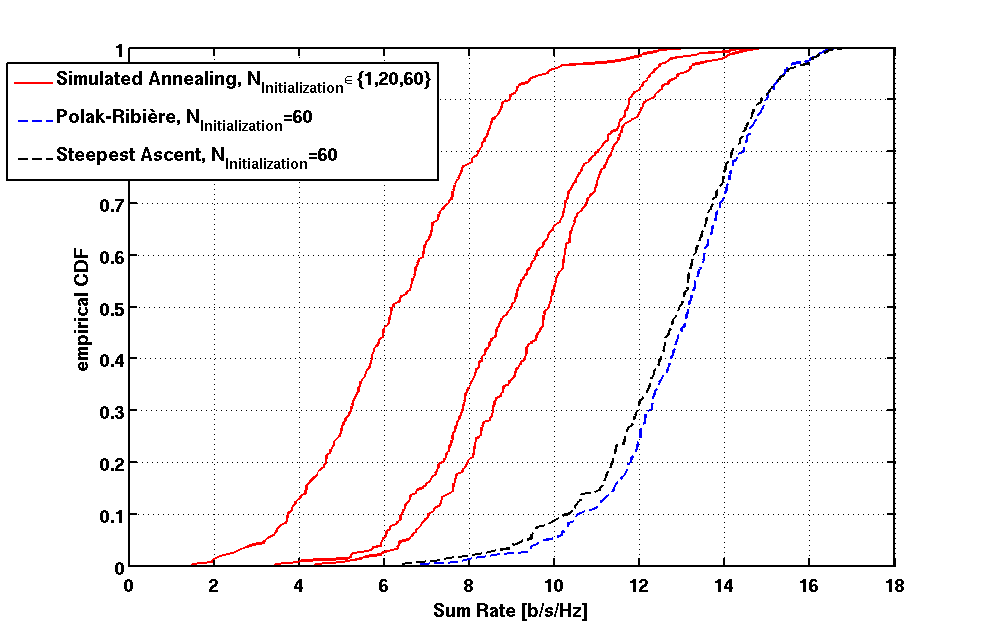
\includegraphics[width=0.8\linewidth]{images/Simannealcomparison.png}
\caption{Comparison of the Simulated Annealing algorithm for different number of initializations and the results from "Polak-Ribi\`{e}re" and "Steepest Ascent" gradient searches.}
\label{fig:heur_sa}
\end{figure}

The Algorithm used in this thesis is a build-in function of MATLAB\copyright.
A description can be found on the MathWorks homepage~\cite{matlab:simulann}.



Figure~\ref{fig:heur_sa} shows the performance of Simulated Annealing algorithm dependent on the choice of numbers of initializations (red curves).
Again we see, that the more initializations we have, the better the sum rate can be optimized.
However, we also see, that even with 60 initializations, Simulated Annealing leads to a result, which is worse than the sum rates achieved by steepest ascend (black dashed curve) and Polak-Ribi\`{e}re (blue dashed curve).


\subsection{GlobalSearch}
\label{sec:globals}
The other two heuristic optimization algorithms are GlobalSearch (GS) and MultiStart (MS).
They are very similar to each other, the only difference is the choice of the starting values.
As MultiStart requires the number of initialization values, GlobalSearch generates trial points on its own~\cite{matlab:gloabls}.
GlobalSearch - the optimization function, which we will analyze - is based on the MATLAB\copyright  built-in function \textit{fmincon}.
Figure~\ref{fig:globals_scheme} shows the schematics of GS and MS.
\begin{figure}[h]
\centering
  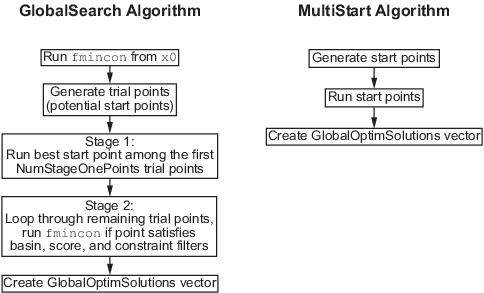
\includegraphics[width=0.5\linewidth]{images/global_algorithm.png}
\caption{Schematics of the GlobalSearch and MultiStart algorithms~\cite{matlab:gloabls}.}
\label{fig:globals_scheme}
\end{figure}

Figure~\ref{fig:globals} shows the performance of GlobalSearch (red curve).
We see, that it has almost the same performance as the conjugate gradient method by Polak-Ribi\`{e}re with 60 initializations (blue curve).
GlobalSearch is less dependent on the initial value - for the relays it is chosen very large ($\vec{X}_{\text{Rel}} = 1000j$) and not at random, compared to the gradient search methods, to simulate an open circuited antenna and therefore no coupling.
\begin{figure}[h]
\centering
  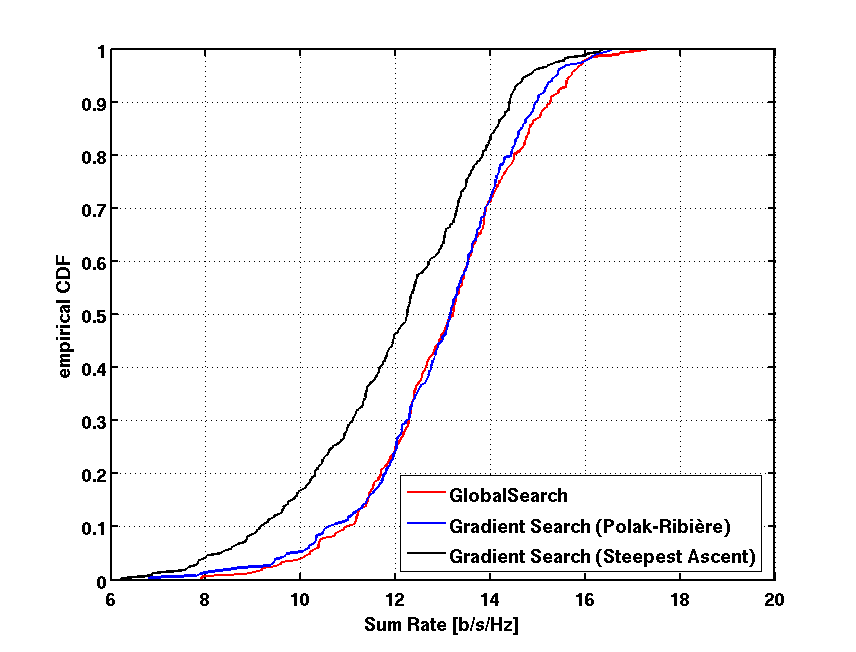
\includegraphics[width=0.7\linewidth]{images/Globalscomparison_edited.png}
\caption{Performance of the GlobalSearch algorithm in comparison to the previous results.}
\label{fig:globals}
\end{figure}

\section{Further Algorithm Improvements}

\subsection{Optimization of the Interference Function}
\label{sec:preoptimization}
A further approach to optimize the gradient search routine is a good initial guess.
The problem of the sum rate maximization is reduced only to the description of the interference.
Therefore the number of variables can be reduced by a factor of two third for the matching network, as the interference function from Equation~\eqref{eq:port_reduction} - even after multiplication with the spatial channel transfer function~\eqref{eq:spatial_channel} - only requires the input impedance of the matching network.
\begin{figure}[h]
\centering
  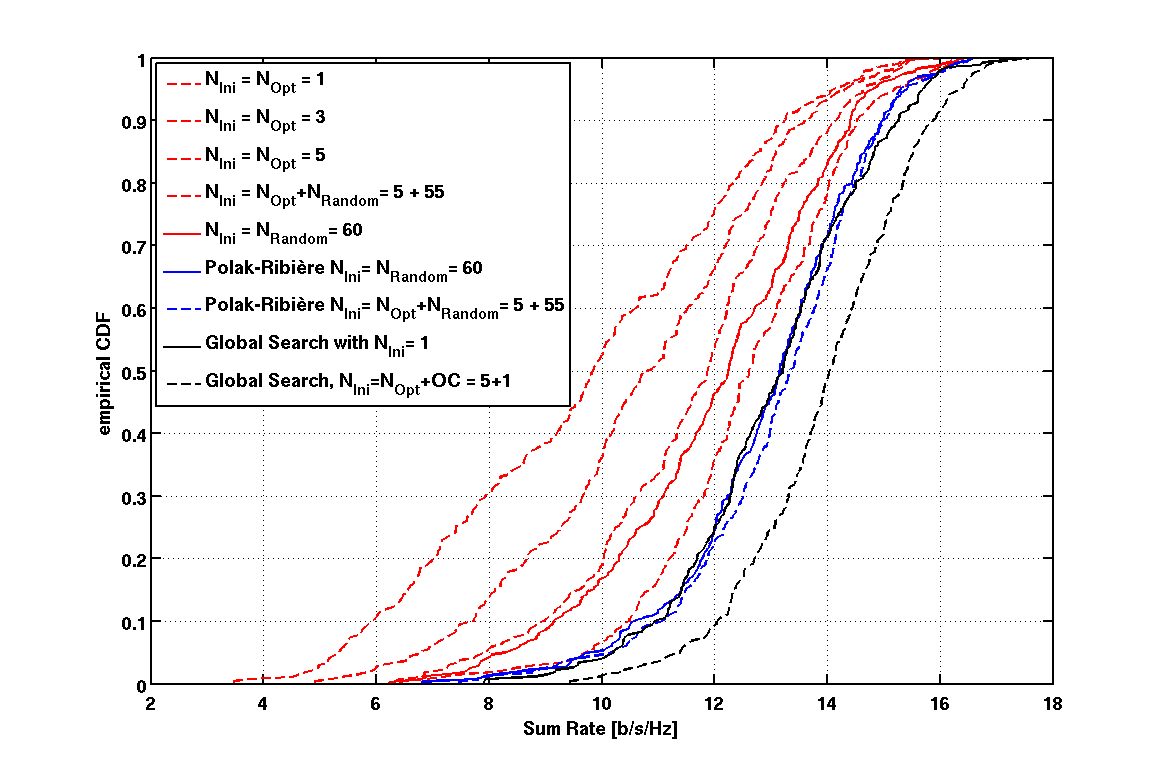
\includegraphics[width=0.9\linewidth]{images/Inioptcomparison_edited.png}
\caption{Comparison of the number of initial values used with different pre-optimized intial values.}
\label{fig:iniopt_comp}
\end{figure}
This reduced problem has size of $N_\text{var} =  2\cdot N_\text{Rel}+2\cdot N_\text{R}\cdot N_\text{Rx} = 2\cdot 4\cdot 5 + 2\cdot 4\cdot 2 = 56$, for the same settings as above.
The factor 2 from the matching network variables comes from the fact, that with pure imaginary elements in the matching network, any complex value of the input impedance can be achieved.


Figure~\ref{fig:iniopt_comp} shows the performance of the steepest ascent algorithm, with the pre-optimized initial values (three red dotted curves on the left).
We see, that using the five best pre-optimizations leads to a performance almost as good as initializing the algorithm with 60 random vectors (red solid curve).
To push the optimization even further, we can combine these two techniques and take the best optimization from the five best pre-optimized initial values and 55 random initial values (red dotted curve on the right).
This leads to a $0.5 \left[\text{b/s/Hz}\right]$ improvement at the mean and a $1.5 \left[\text{b/s/Hz}\right]$ improvement for the lowest 10\% of the rates, than only considering random values.

Applying this to the method of Polak-Ribi\`{e}re (blue dotted curve), however, does not improve the results as much as with the steepest ascent method.
A sum rate of only about $0.1 \left[\text{b/s/Hz}\right]$ higher is achieved by using pre-optimized initial values in combination with the method of Polak-Ribi\`{e}re.

Finally, this method is applied to the heuristic GlobalSearch routine.
As mentioned in Section~\ref{sec:globals}, GloablSearch is less dependent on the initial value and therefore, the initial value is chose to be open circuited for the relays.
With five optimized initial values plus the standard open circuit initial value, an improvement of almost $1.0 \left[\text{b/s/Hz}\right]$ can be achieved (black dotted curve) compared to initializing only by the open circuited value (black solid curve).


\subsection{Post Refinement of GlobalSearch by Gradient Search}
\label{sec:postrefinement}
When the problem of gradient search is, that it may run into non optimal local maximas, the questions remaining for the heuristic solvers are: "How good are the results after all?" and "Can they be improved any further?"

\begin{figure}[h]
\centering
  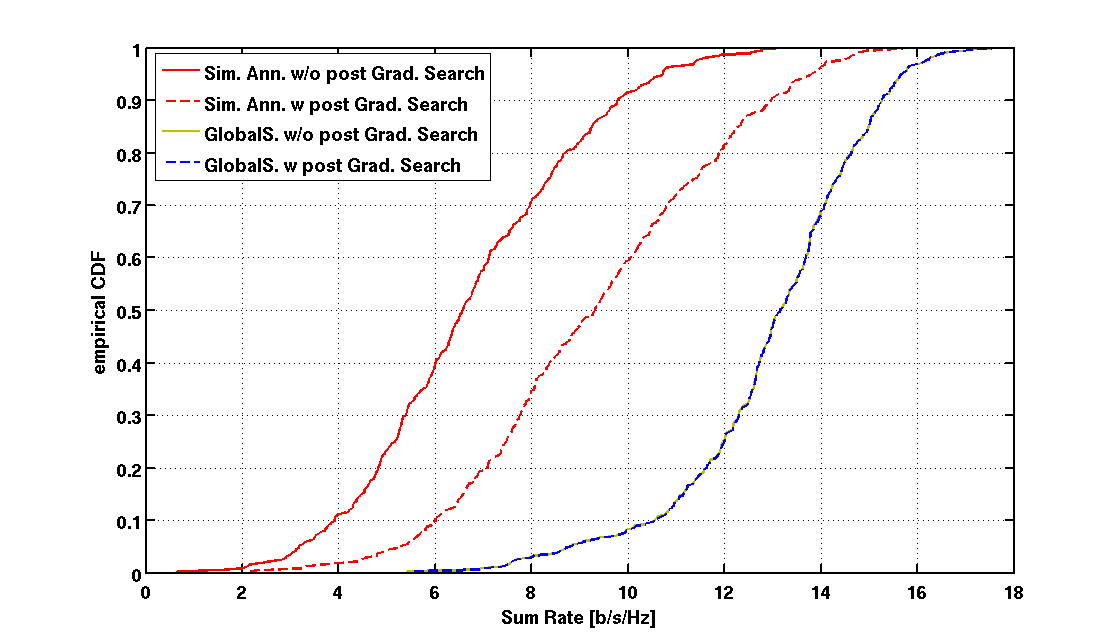
\includegraphics[width=0.9\linewidth]{images/Postrefinementcomparison.png}
\caption{Comparison the heuristic solvers with and without a post refinement by gradient search.}
\label{fig:postrefinement}
\end{figure}

The approach in finding the answers, is to use the gradient search routine on top of the heuristic solvers as a refinement.
Figure~\ref{fig:postrefinement} shows the performance of the Simulated Annealing and the GlobalSearch algorithm (solid red and solid yellow curves).
The dashed lines show the result, when gradient search was added on top of the heuristic solvers (red for Simulated Annealing and blue for GlobalSearch).
This shows, that the poor results of the Simulated Annealing algorithm does not lead to any good initial value for the gradient search as after the refinement the performance is still about $5 \left[\text{b/s/Hz}\right]$ worse, than the performance of GlobalSearch.
Second, it shows that the performance of GlobalSearch is quite good, as any post refinement of gradient search \emph{does not lead to any significant improvement}.


\subsection{Stepwise Optimization}
\label{sec:stepwise}
In the previous Sections, we saw the performance of different methods for three relays per user.
The number of relays was kept small for the analysis of the algorithms, so that complexity effects diminishing the performance were avoided.
Increasing the number of relays might result in worse sum rates as the complexity of the system correlates with the number of required initial values to achieve similar good results, hence the run time of the solver must be increased, or the precision is decreased.
Therefore we will have a look at the performance of the optimization and how it can be pushed in the following.
For the results shown below, the number of relays were increased to seven, if not mentioned specifically.

In Figure~\ref{fig:nrel7} we see the performance of the GlobalSearch algorithm, optimizing a 2x2 MIMO system, with seven relays and one receiving antenna per user (red curve).
The black curve shows the performance of the algorithm optimizing only three relays per user (c.f.  red curve in Figure~\ref{fig:globals}).
Actually this should be a lower limit of the red curve, as one solution for seven relays is to optimize only three of them and open circuit the remaining four.
However this is only the case for about 85\% of the cases, the lowest 15\% actually lead to a worse solution than only optimizing three relays.
This shows, that the GlobalSeach optimization might not perform very good on larger problems, i.e. reducing the size of the problem results in a better sum rate.

\begin{figure}[h]
\centering
  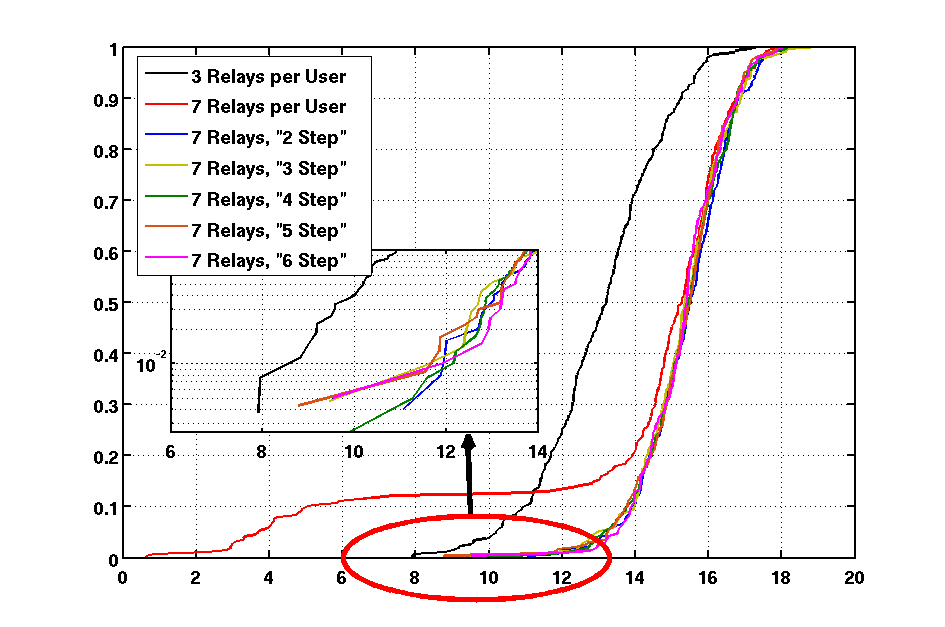
\includegraphics[width=0.9\linewidth]{images/Relstepcomparison_edited.png}
\caption{Comparison of the number of step wise optimization.}
\label{fig:nrel7}
\end{figure}

Therefore one approach to prevent GlobalSearch of running into a low rate, is to reduce the number of relays to optimize and increase them stepwise.
The blue curve shows to result of the optimization, when GlobalSearch is allowed to optimize only two relays.
Once finished, two additional relays are considered so that in total four relays per user are optimized.
This is repeated until the total number of relays is reached (in this case four times, $N_{\text{Rep}} = \lceil\frac{N_{\text{Relays}}}{N_{\text{Step}}}\rceil = \lceil\frac{7}{2}\rceil=4$).
This leads to a tradeoff between the precision of the routine and the run-time, as a smaller number of relay steps ($ N_{\text{Step}}$) will lead probably to a better result, but also to a larger number of repetitions and therefore it will take a lot longer ($\approx N_{\text{Rep}}*\text{T}_0$, for $\text{T}_0$, the time for one optimization).

\begin{figure}[h]
\centering
  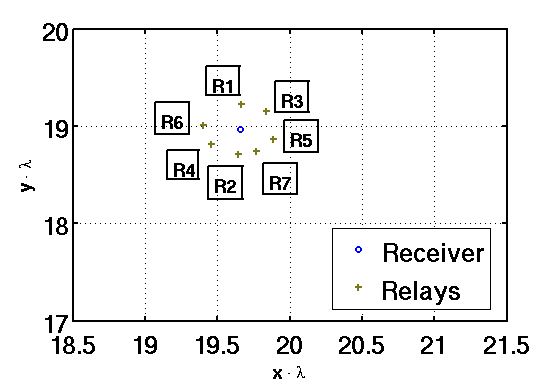
\includegraphics[width=0.6\linewidth]{images/choice_of_relays.png}
\caption{Example of choosing the relays for stepwise optimization.}
\label{fig:rel_choice}
\end{figure}

The first relay is therebey chosen at random.
For the following relays, the algorithm takes always the next free relay across the receiver.
Figure~\ref{fig:rel_choice} shows an example on how the relays would be chosen for this setting.

Back in Figure~\ref{fig:nrel7}, the yellow curve shows the optimization for a stepwise increment of $N_{\text{Step}}=3$.
Therefore $N_{\text{Rep}} = 3$ had to be taken.
As for $N_{\text{Step}}=4$, $N_{\text{Step}}=5$ and $N_{\text{Step}}=6$ (with each $N_{\text{Rep}} = 2$), it leads almost to the same result.
It can also be seen, that none of the stepwise optimized solvers has a significant low rate outlier (logarithmic scaled subplot), therefore we can say, that the outliers from the direct optimization can be avoided, when a single repetition is added.

A second approach is to optimize one user and its relays per step.
This reduces the size of the problem to $N_\text{R}\cdot N_\text{Rx}+N_\text{Rel}$ for each optimization step.
The number of optimization steps is increased by $N_\text{R}$.
Additionally after optimizing each user a final step might be included, where the whole system is refined.
\begin{figure}[h]
\centering
  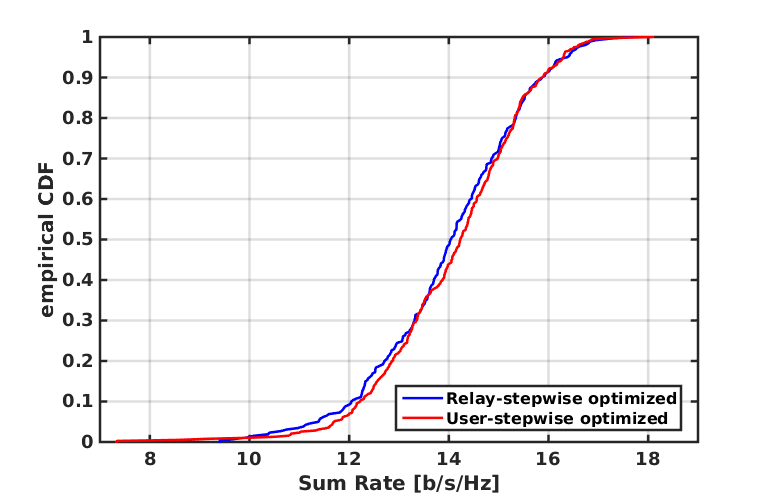
\includegraphics[width=0.9\linewidth]{images/stepwise_comparison.png}
\caption{Comparison of optimizing the relays stepwise versus optimizing each user per step.}
\label{fig:uservsrelay_stepwise}
\end{figure}

Figure~\ref{fig:uservsrelay_stepwise} shows the performance of this method for a $2\times2$ system with three relays per user.
The blue solid curve denotes the performance of optimizing the system directly.
The red solid curve shows the performance of optimizing each user on its own and additionally optimizing the whole system in a refinement step afterwards.
It can be seen that optimizing each user in advance of optimizing the whole system, leads to a slight improvement, even for this small system.

For both cases - the user stepwise optimization and the relay stepwise optimization - a lower sum rate limit constraint is set after each step.
With this inequality constraint, the heuristic algorithm is prevented in running into a lower rate than in the previous step.


%The main difference are the rates below $12 \left[\text{b/s/Hz}\right]$ (logarithmic scaled subplot).
%Whenever the step to increase the number of relays was chosen to be even (i.e. on both sides of the relay were the same number of relays optimized), the rates were higher.
%This speaks for some symmetry in optimizing the relays.
%Additionally, the lower the size of the "step" (i.e. the higher the number of the repetition), the higher were the optimized rates (c.f. "3 Steps" (yellow) and "5 Steps" (orange), or "2 Steps" (blue) and "4 Steps" (green)).




